% Preserving Code Review Comments Across Revisions (team02, edition v05), 15 pages, IEEE two-column.
% All tables are LaTeX; the two diagrams are PNG files in assets/ (captions are part of the images).
% Reported values are generated by the public artifact; see ../README.md for the macro behind each table.
% Study scope: public data only; private repository histories and selected student repositories are excluded.
% Bibliography: 41 entries ordered by first citation, November 2026.
% Compiles with pdfLaTeX (Overleaf default) or XeLaTeX; run twice.
\documentclass[10pt,conference,letterpaper]{IEEEtran}
\usepackage{iftex}
\ifPDFTeX
  \usepackage[T1]{fontenc}
\else
  \usepackage{fontspec}
  \IfFontExistsTF{Tinos}{\setmainfont{Tinos}}{\setmainfont{TeX Gyre Termes}}
\fi
\usepackage{booktabs}
\usepackage{graphicx}
\usepackage{amsmath,amssymb}
\usepackage{url}
\usepackage[hyphens]{xurl}
\usepackage{hyperref}
\usepackage{microtype}
\usepackage{tabularx,array}
\hypersetup{hidelinks}
\newcolumntype{L}[1]{>{\raggedright\arraybackslash}p{#1}}
% relocation and issue-state labels are set in sans-serif, as in the figures
\newcommand{\lbl}[1]{\textsf{#1}}
% footnote under a table, set to the float's width
\newcommand{\tablenote}[1]{\par\smallskip\parbox{\linewidth}{\footnotesize #1}}
\title{Preserving Code Review Comments Across Revisions}
\author{\IEEEauthorblockN{Raisa Jose, Noel Alex Samuel, Khadheeja Safar, and Kalyanaraman P}
\IEEEauthorblockA{School of Computer Science and Engineering,\\Vellore Institute of Technology, Vellore, India}}
\begin{document}
\maketitle
\begin{abstract}
Comments should continue to be linked to code even if they have been moved. We distinguish between code changes, valid linking, and issue resolution. To achieve this, we provide location-independence by providing quotation-based change markers, indentation, and copy protection, as well as prohibiting resolution through movement. We evaluated on controlled edits made to code. The evaluation used 5 public python repositories with a total of 8,805 uniformly sampled and 2,454 targeted observations. It also used an independent benchmark with regions annotated by humans (200 regions), synthetic tests (23,550) and 998 suggested changes from public GitHub repositories in 5 languages. 4 sets of private histories and 20 selected student repositories were not used. The controlled and constructed suites use author-derived source files. In public targeted histories, the cascade had 1,639 correct location/absence predictions (1,639/2,454 = 66.8\%). The cascade achieved 72.5\% change classification. However, 17 of 1,930 required rechecks were missed. Compared to the cascade, CodeMapper performed better in the independent manually annotated benchmark (91.5\% correct line/absence against 66.0\%). In synthetic cases, adding 2 protections to CodeMapper reduced missed rechecks from 19.3\% to 3.1\%, although unnecessary requests increased from 13.4\% to 37.0\%. Exposed changes occurred in the change suggestion outside the quotations. Some previous aggregated results on protection and longitudinal data could not be provided on just public data without re-running traces. The bounded model reveals missing points in the life cycle of issues. It also defines a stronger contract than has been implemented. Within the data provided, the work is technically viable. However, its effect on the workload of supervisors or students has not been measured.
\end{abstract}
\begin{IEEEkeywords}
Code review, anchored annotations, Source code tracing, Software evolution, Language models
\end{IEEEkeywords}
\section{Introduction}


In this scenario, either locations of comments change (but concerns remain) or concerns are resolved with mostly unchanged quoted text. Across 5 open source Python projects, 601 (64.6\%) (95\% CI: 57.9\%--70.8\%) of 931 inline review comments in merged PRs have been aged in GitHub. Of the aged comments, 99.0\% had no position in the diff. Therefore, while the comment is visible to the reviewer, they cannot see where it now resides. In Living Review (resubmission mode of the capstone review portal described in Section IV), faculty supervisors add concerns to a team’s code across multiple versions. Suppose in version 1, a supervisor adds a concern in client.py about a retry loop never backing off. In worker.py, there is an exact copy of this loop. In version 2, this loop is fixed in client.py, but not in worker.py. Using quotation-based location, there is no match for the quoted text. Instead, the text is matched in its exact form in worker.py, and a change of location is reported. The supervisor sees an old concern on unchanged code. As there is no evidence within the comment itself that the code being concerned changed, the supervisor may decide to resolve or dismiss this concern, without seeing any changes. This is an example of the exact copy issue explained in public histories and constructed tests (Section VII). If using GitHub, this would be marked as aged, and the position removed. However, using the proposed method for this issue, although the candidate position is preserved, there is evidence that this quoted text was present in worker.py, and therefore re-checking is requested. The quoted text from review and current text are shown together, and issue is left open until the supervisor makes a decision. The deployed application uses the unguarded cascade (Section IV). This example shows three properties of interest in feedback persistence, often conflated in tooling. Whether the reviewed code changed, whether the anchor is valid, and whether the issue is unresolved by the supervisor. The first two are properties of code, and can be quantified. The third is only known by the supervisor. Whilst a change in this code is indicative that the issue may have been impacted, it is not definitive proof of resolution. Although recent literature has explored feedback literacy \cite{lei2026,istencioglu2026,little2024,carlessyoung2025}, it is unclear if feedback persistence helps supervisors provide re-reviews and students enact feedback. Studies in feedback literacy in practice indicate that ‘taking up’ feedback is an active student behaviour \cite{woitta2025,zheng2026}. This paper investigates the technical challenges, and conditions between issues and supervision, but does not quantify learning, re-review times, or outcomes for workload. Research into annotated code regions has addressed persistence of locations and tracking changes \cite{meta2024,magic2024,codetations2026,codemapper2026}. Comments are also automatically ported/aged on existing review platforms according to product specific criteria. Empirical studies in code changes during reviews, and analysis of their impact, highlight that finding changes to code does not necessarily mean we know why the change was made, or if it was sufficient \cite{fregnan2022,gocmen2025}. We make no novel ideas on matching, with the matching algorithm of the portal not being optimal. The contribution is safe feedback persistence. It provides a contract for feedback persistence where evidence of relocation may only progress an issue towards resolution by the supervisor (5 requirements) and a safe layer to apply this contract to any location algorithm. When relocating, labels of change are calculated based on the quoted text. Two guards check the output of the relocated window. The quoted text is preserved, and no relocation resolves the issue. The safety layer guarantees S1--S3 only under explicit assumptions. If the exact code occurs in a copy, the code is normalised, or changes occur in code around an unchanged quote, re-checking may still be evaded. In the existing application, issues can only be removed from review by manual deletion, or auto-generated dismissal. S4/S5 therefore do not hold at this stage of the lifecycle. The stronger contract is verified by model checking but has not yet been implemented (Section VIII). As the safety layer only considers the output of the location window, it can be applied to a stronger region mapping algorithm, or language model. Issues can result in: Misleading supervisors (wrongly located), or search by the supervisor (no location). Therefore, primarily the safety issues are: failure to re-check, changed/deleted code not returned to supervisors, and silently misplaced. Misplaced issues, misleading requests, invalid anchors, and unnecessary rechecks waste effort. All configurations are reported with these issues, and location accuracy. For each outcome, counts are given with different denominators. Acceptable rates are a decision to be taken in practice, therefore trade-offs are presented. RQ1 Location: How accurate are the cascading methodology, standard review practices, contextual line tracking, region mapping and language models at locating code anchored in reviews from controlled changes, 5 public Python projects, independently annotated benchmark, and applied review suggestions in 5 languages? RQ2 Safety Layer: How frequently is changed code not returned to supervisors, or issues silently misplaced? What mechanisms cause these issues? How much less frequent are these issues (when using a location agnostic layer), for all location methods, and what is the cost? What tradeoffs exist in applying a configuration to new code? RQ3 State Contract: Does the implemented lifecycle adhere to S4 and S5? What must be done to enable a contract to adhere to S4 and S5? Contributions: 1) Feedback persistence contract. Three properties of interest, 5 safety requirements (with assumptions), and counterexamples in each of the failure mechanisms found (Section III-E). Comparison with other review tools and tracking systems on each requirement (Section II). 2) Feedback persistence safety layer, allowing the contract to be applied to any location method, integrated with the deployed portal (which only uses the cascading methodology as a system of record). Guards and identity rule have been evaluated, but not yet implemented (Sections III--IV). 3) Evaluation on controlled data, public data, and independently annotated data, all with strength of evidence. An oracle was created from applied review suggestions, and all 6 outcomes defined have evidence from archived data. Experiments include removing guards and exact copy placement, and experimenting with different guard selection and exact copy placement. (Sections V--VII). Negative results: Evidence of change in the text from the language model is unsafe. A provenance-based exact copy guard does not work well in tests with many copies. The guards identify incorrectly located issues but do not resolve them. Insertion around unchanged quoted text can be evaded by all location methods. 4) The implemented lifecycle was verified using static scanning, bounded model checking and scenarios. A stronger contract was designed to address gaps in the implemented lifecycle. (Section VIII). The extended artifact discussed previously also includes analyses of mixed histories. Only explicitly mentioned populations in this section support this edition of the artifact.








\section{Background and Related Work}

\textbf{Robust annotation anchoring.} Stable linking: Several tools have been developed to associate annotations with changing code. Meta-Manager tracks edits on the annotated code \cite{meta2024}. Magic Markup provides re-tagging using a language model \cite{magic2024}. In peer-reviewed work, Codetations tracks edits locally and matches annotations based on their semantics to allow annotations to be applied to changed code offline \cite{codetations2026}. CodeMapper identifies arbitrary regions of code between commits through diff matching, identifying motion, and searching \cite{codemapper2026}. However, none of these solutions can confirm that a concern raised by a supervising academic has been fixed.

\textbf{Code review and warning tracking.} With modern code reviews becoming increasingly automated \cite{roadmap2026}, empirical studies reveal many aspects to consider in their quality. For example, review comments address both understandability and bugs \cite{oliveira2025}. However, after review, security issues may still be left uncovered \cite{charoenwet2024}. Furthermore, changes may be made to code during review which may not be directly related to comments given \cite{fregnan2022}. Within the field of code review communication, it has been shown that code review is more than simply detecting bugs, and involves exchanging information between people \cite{dorner2025}. CodeReviewQA considers how LMs reason about different code revisions. It identifies where in code changes should occur \cite{codereviewqa2025}. In a peer-reviewed qualitative study of automated code reviews, Tufano et al. identified several success and failure scenarios, and various issues within the evaluation data \cite{tufano2024}. Language model code review systems also include filtering and feedback mechanisms \cite{bitsai2025}. Recent studies show that pre-processing may impact the result of automatically suggested code changes \cite{pirouzkhah2026}. Therefore, it makes sense to verify suggestions against evidence rather than taking decisions based on the model’s outputs. To track static warning information, work has been done to ensure warnings can be tracked across code changes \cite{warnings2024}. ViolationTracker allows accurate tracking of violations with different statuses: introduced, resolved, removed and reopened \cite{violation2023}. If a static analysis finding no longer exists, then it can be considered resolved. However, if a concern raised by a supervisor remains unresolved, it cannot be resolved according to this rule. Different policies exist in GitHub and Gerrit for out-of-date review opinions, as summarised in Table~I. The specific details provided in this table for each product do not represent peer reviewed experimental findings.

\textbf{Code change versus review resolution.} Change not satisfaction. Whether changes were made in response to feedback, and whether these satisfied the concerns raised by supervisors are two distinct questions. This is not a statement on whether semantic correctness can be inferred from source code similarity. Applying the ‘changed’ label will result in further inspection, it will never close or maintain a concern. In evidence from interviews, trust and context are identified as barriers to using feedback generated by AI tools during code reviews \cite{alami2025}. Similarly, recent work in pull requests including AI has found variation in human involvement and interaction, reinforcing the need to consider how humans behave in these scenarios \cite{gao2026,njoku2026}.

\textbf{Differencing and region mapping.} The text matching algorithm used in this system is provided by Python. Contextual line mapping is implemented using a hybrid approach from the LHDiff family of line tracing algorithms \cite{lhdiff2013}. The syntax tree baseline uses GumTree. The algorithm for AST difference computation was published in \cite{gumtree2014} (ASE 2014). Specific implementations and versions used can be found in the reproducibility information. Recent academic research has improved syntax tree differencing in refactoring scenarios, and mapping techniques have been benchmarked \cite{astdiff2024}. Method level traceability has been implemented in CodeShovel \cite{codeshovel2021}. Further work has implemented method and variable traceability \cite{methodtracking2022}. Structural equivalence between blocks during refactorings has been traced \cite{blocktracking2024}. ReCite fixes outdated references to methods in comments within source code \cite{recite2026}. In general these aim to provide mappings, but if mapping uncertainty occurs, what should be communicated to reviewers? Recent literature reviews have looked into using language models to improve quality in code, including fixing and refactoring \cite{alomari2026}, and empirical evaluations have evaluated fixing approaches to remove defects in code quality \cite{patcas2026}. However, these do not replace supervisor validation that a concern raised in prior reviews has been resolved.

\textbf{What is established and what is new.} Existing Features. Discussion tools, warning markers and recent annotations provide stateful feedback. New features. There are no new algorithms in this feature. In this feature, stateful feedback is supported by: 1) an agnostic check system, 2) explicit uncertainty, and 3) an issue statefulness guarantee. However, the implementation of stateful feedback in this feature does have deletion and rejection exceptions. A stronger guarantee is simply proposed, and has been validated. The differences between guarantees are shown in table I. The motivation for providing usable feedback in this feature is given by recent literature \cite{lei2026,istencioglu2026,zhan2026}, and a review of automatic programming feedback \cite{surveyfeedback2025,surveygrading2024,feedbacktypes2026}. This does not show any benefit to using this level of feedback repositioning. This needs to be explored through further research with staff and students. Possible methods for research can be found in education research. A validation study can identify attitudes and approaches to feedback \cite{woitta2025}. A learning analytics study has shown that feedback literacy acts as a moderator on how students perceive detailed feedback \cite{weidlich2025}. A study with multiple feedback interventions has measured student behaviour related to feedback \cite{zheng2026}. None of these have considered this code anchoring approach.

\begin{table*}[!t]
\caption{Review-Persistence Requirements}
\label{tab:review-comparison}
\centering\scriptsize
\setlength{\tabcolsep}{3.1pt}
\renewcommand{\arraystretch}{1.12}
\begin{tabularx}{\textwidth}{>{\raggedright\arraybackslash}p{0.15\textwidth}*{6}{>{\raggedright\arraybackslash}X}}
\hline
Requirement & GitHub$^{a}$ & Gerrit$^{b}$ & CodeMapper \cite{codemapper2026} & CodeTracker \cite{blocktracking2024} & ViolationTracker \cite{violation2023} & Living Review \\
\hline
Arbitrary-line-span anchors & yes & yes & yes & no: code block & no: analyzer warning & yes \\
Follows edited code & not always: outdated thread & ports to calculated position & yes & yes & matches warnings & any locator \\
S1: signals change since review & outdating hides position & ported comment need not signal change & no review-state rule & tracks block history & not applicable & request from original quotation \\
S2: flags ambiguous placement & no mapped position & file-level fallback & no review-state rule & no review-state rule & no review-state rule & copy guard can request re-check \\
S3: makes absence visible & outdated comment & file-level fallback & no match & block removed & deleted warning & removed, re-check \\
S4: only a supervisor closes & human resolves & human resolves & not applicable & not applicable & analyzer may call warning fixed & nominally yes; dismissal exception \\
S5: keeps an open concern across versions & old thread remains & unresolved comment carried & not applicable & not applicable & no human-concern lifecycle & not yet: three gaps \\
\hline
\end{tabularx}
\vspace{2pt}
\parbox{\textwidth}{\footnotesize Vendor behavior is a documented product policy, not a peer-reviewed result or a measured comparison. $^{a}$ GitHub, “Precision review comment outdating,” Sep. 25, 2018: \url{https://github.blog/changelog/2018-09-24-precision-review-comment-outdating/}. $^{b}$ Gerrit, “Porting Comments User Documentation,” current documentation: \url{https://gerrit-review.googlesource.com/Documentation/user-porting-comments.html}. Both consulted Nov. 18, 2026. The implementation currently has documented S4 and S5 gaps, as analyzed in Section~VIII.}
\end{table*}


\section{Design}


\subsection{Versions, Anchors and the Cascade}


An input submission, $V_t$, includes files $(\pi,T)$ and extracted text. An anchor, $a=(\pi,s,e,c,q)$, references a file, and includes the first/last line numbers (s/e), the full SHA-256 checksum (c) and quoted text (q). It spans $k=e-s+1$ lines. Lines of q with non-zero non-whitespace characters are included in $\bar q$. Quotations can be used to match evidence, but do not represent unique identifiers for individual program elements. Multiple (up to 12) anchors can exist per issue. Re-location results in a new location and label. Tier 1 searches the original digest. Tier 2 searchs in the same file for occurrences of $\bar q$ (with all whitespace removed, and only non-zero lines). The best match is chosen closest to the previous start position. Tier 3 predicts a new start line using a line diff. Candidate windows of size $k$ are considered at positions $p\pm r$, where $r=\max(10,2k)$ and $p$ is the predicted line. For each window, similarity is calculated as $2\sum_i m_i/(|u|+|v|)$ where $m_i$ is the length of matching blocks. If the best window has a ratio $\geq\theta$ (default: 0.85) it is selected. Tier 4 searches in other files. Fuzzy searching is performed in the current file first to avoid bias towards identical copies found in other locations.





\subsection{Labels and Their Limits}


Normalization allows issues to remain as anchors despite changes in blank lines and layout. However, in Python indentation is meaningful. If a line becomes un-indented from a conditional clause, although the text may be normalized, the meaning of the line has changed. Thus, content match and moved are based purely on text matches. Another limitation is the possibility of duplicates. If a duplicate of this issue exists elsewhere, and if the original is edited/deleted, then tier 2 and 4 may return a moved status.


\begin{table}[!t]
\caption{Relocation Labels}\label{tab:labels}
\centering\footnotesize
\setlength{\tabcolsep}{3pt}
\begin{tabular}{@{}L{.17\columnwidth}L{.37\columnwidth}L{.24\columnwidth}L{.12\columnwidth}@{}}\toprule
Label & Holds when & Does \emph{not} establish & Issue \\ \midrule
\lbl{identical} & same path and same file digest (tier 1) & semantic review of the file & keeps state \\
\lbl{content-match} & normalized quotation $\bar q$ found at the old start (tier 2) & byte identity, equal indentation, equal behavior & keeps state \\
\lbl{moved} & $\bar q$ found at another start or in another file (tiers 2, 4) & that the match is the original copy & keeps state \\
\lbl{changed} & best near-predicted window has ratio $\ge\theta$ (tier 3) & that the concern is affected & re-check \\
\lbl{removed} & no tier succeeds & that the code was deleted & re-check \\ \bottomrule
\end{tabular}
\tablenote{The deployed code emits a single identifier, \texttt{exact}, for both \lbl{identical} and \lbl{content-match}; this paper separates them because only the first is a byte-level property. Normalization strips each line's leading and trailing whitespace and skips blank lines.}
\end{table}


The status of the issue remains unchanged by this edit, and thus the change will not be returned to the supervisor.


\subsection{The Safety Layer}


Two guards, labels, and conditions on issues are used in this stage. Both guards use protocols whose text and code hash values are known prior to running the held-out runs. The cascade used in practice is therefore the system.


• Indent guard (IG): If the run is accepted, the indentation widths of non-empty lines are compared to those of the quote, relative to the initial line, and in absolute terms. In Python, if there are any differences, then the label of the run will be changed. In other languages, only relative differences cause the label to change.


• Copy guard (AGi): If the run is accepted at any position other than an expected position, the number of instances of $\bar q$ in the old and new versions of the candidate file are counted.


\begin{figure*}[!t]
\centering
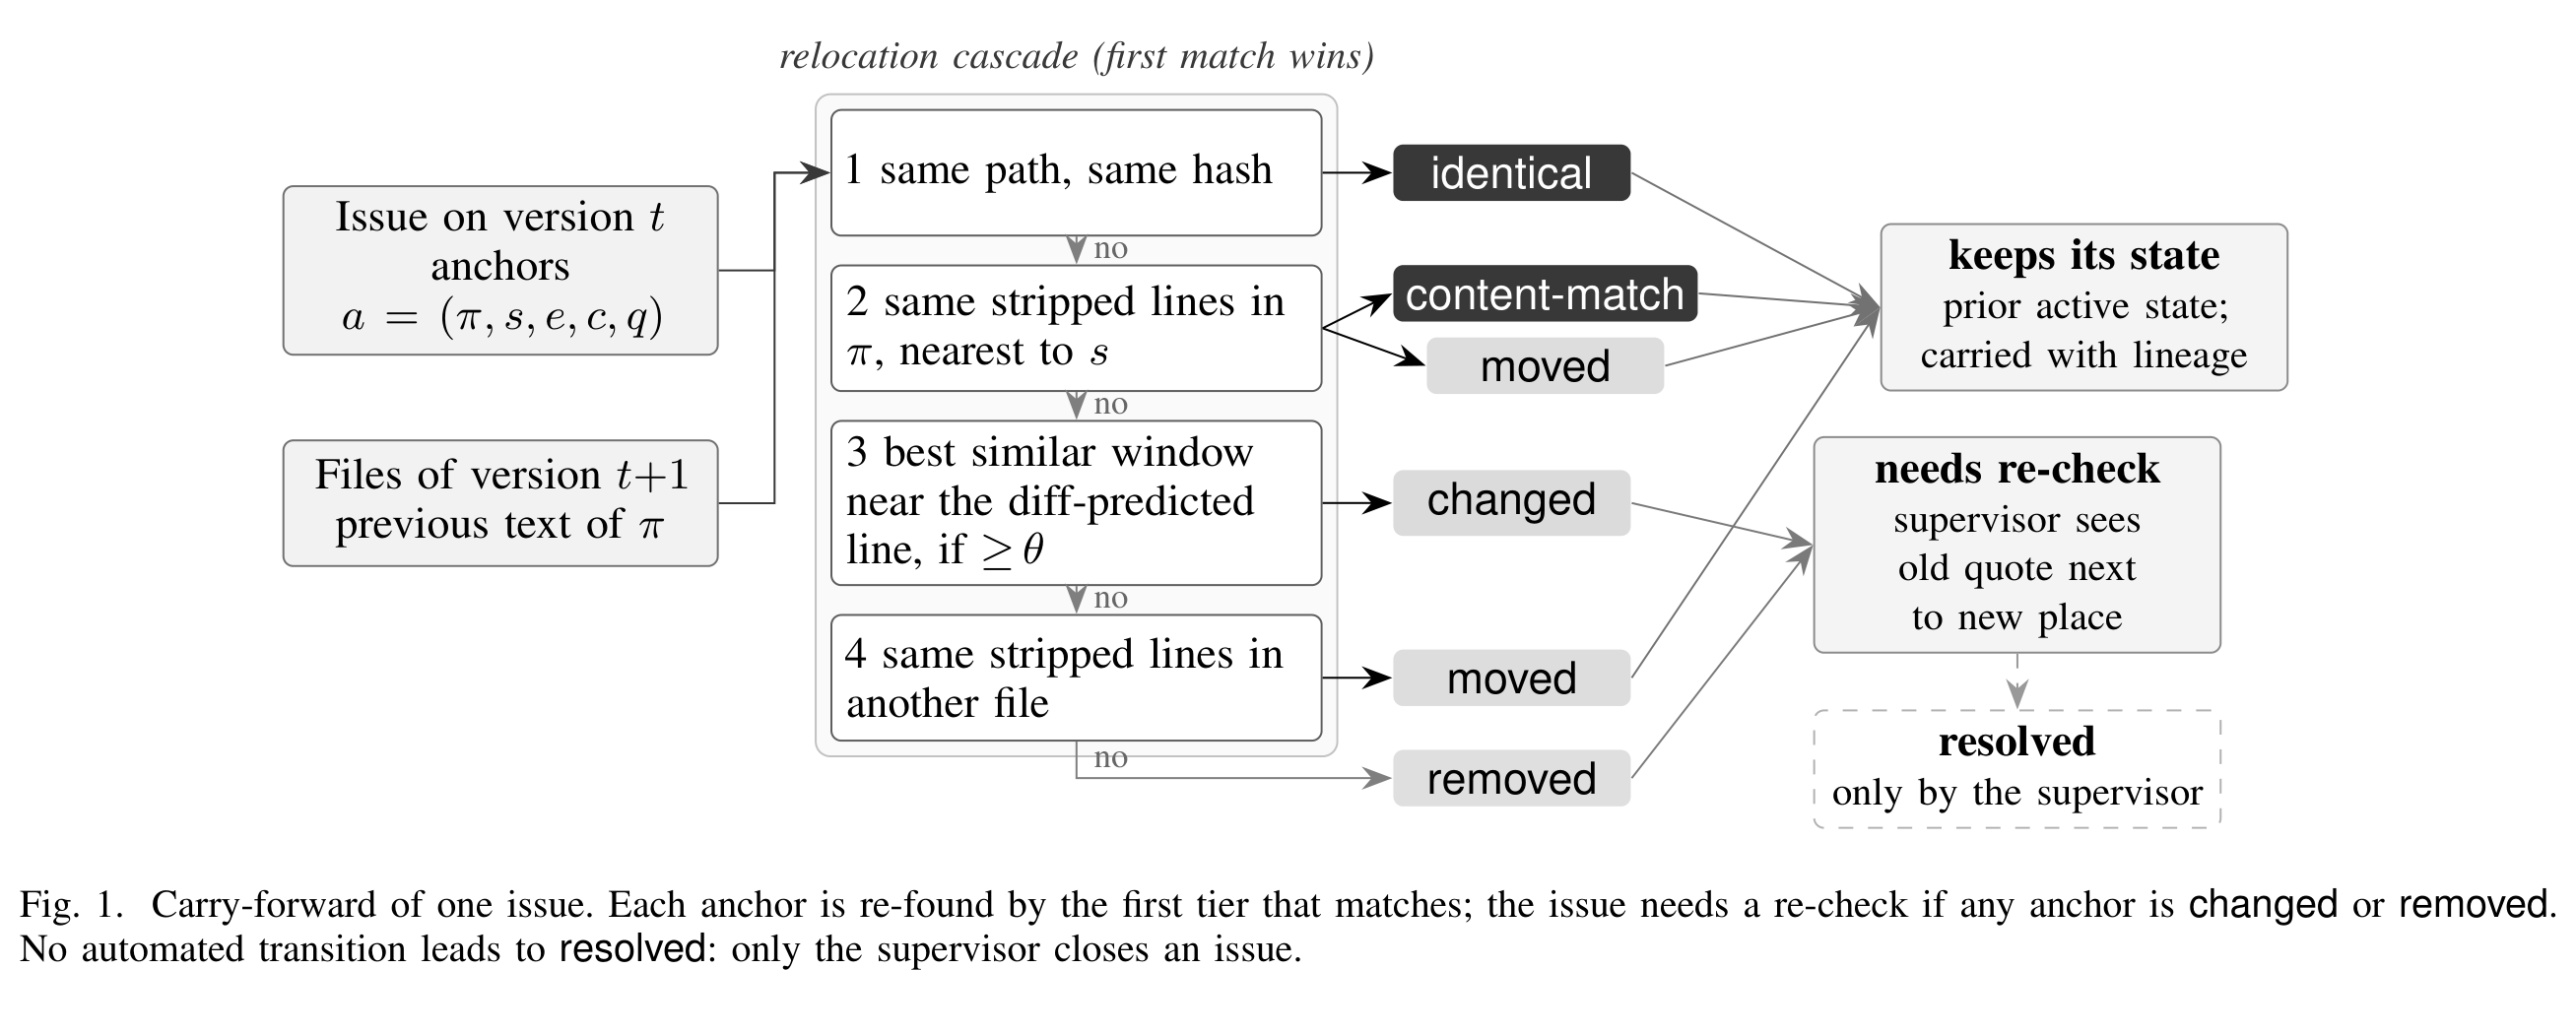
\includegraphics[width=\textwidth]{assets/figure_1.png}
\end{figure*}


If the text was truly copied, only increases in the number will produce a clean copy. Otherwise, the position is maintained, but rechecking is requested. The original version of this guard (AG) marked a clean insertion immediately above an anchoring point as true (as the anchored portion of the diff is mapped from the original anchoring position in the old file to the first inserted line of the new file). AGi allows the line to which the anchoring position’s first line is mapped as an expected position.


• Variable width window (VW). In tier 3, windows of height $k+d$ and $k-d$ ($d=\max(1,\lceil k/2\rceil)$) are scored so that growing/shrinking statements are recovered at their new size. This is part of the search performed by the cascade.


• ID rule (ID): If tier 3 returns an altered window, then the quoted text at the anchoring point is replaced with the matched text. Any incorrect fuzzy match means that all future versions will be based on the incorrect match. The original quoted text $q_0$ (as seen by the supervisor) is retained, as well as the current quoted text $q_t$. If the text has moved, then $q_t$ is still tracked. However, for every altered hop, similarity to $q_0$ must be at least 0.5. If not, then it is reported that the anchor has been removed. Requests are made with reference to $q_0$. If any of the located code is different to what was seen by the supervisor, then an issue is raised. This stage only requires the window returned, and old and new versions of the file to be known (so applies to any output of locators). None of these prove identities. Two copies in the same revision cause AGi to fail. IG indicates style equivalence, rather than equivalence. The provenance rule (AG2) which accepts a window based on where the lines came from in the diff is a negative result (see Section VII). It is impossible to determine which of two identical copies was seen in review just from content. It is only possible to know when to request.


\subsection{Issue States}


In a new version, issues (open, accepted or under review) from the previous state are carried forward. Anchors are moved to point to the new location, and the lineage relationship is added. If anchors have changed or been removed, the issue is put under review. Otherwise, the issue remains in its previous state as normal. Issues cannot be resolved in relocation transitions.


\begin{figure}[!t]
\centering
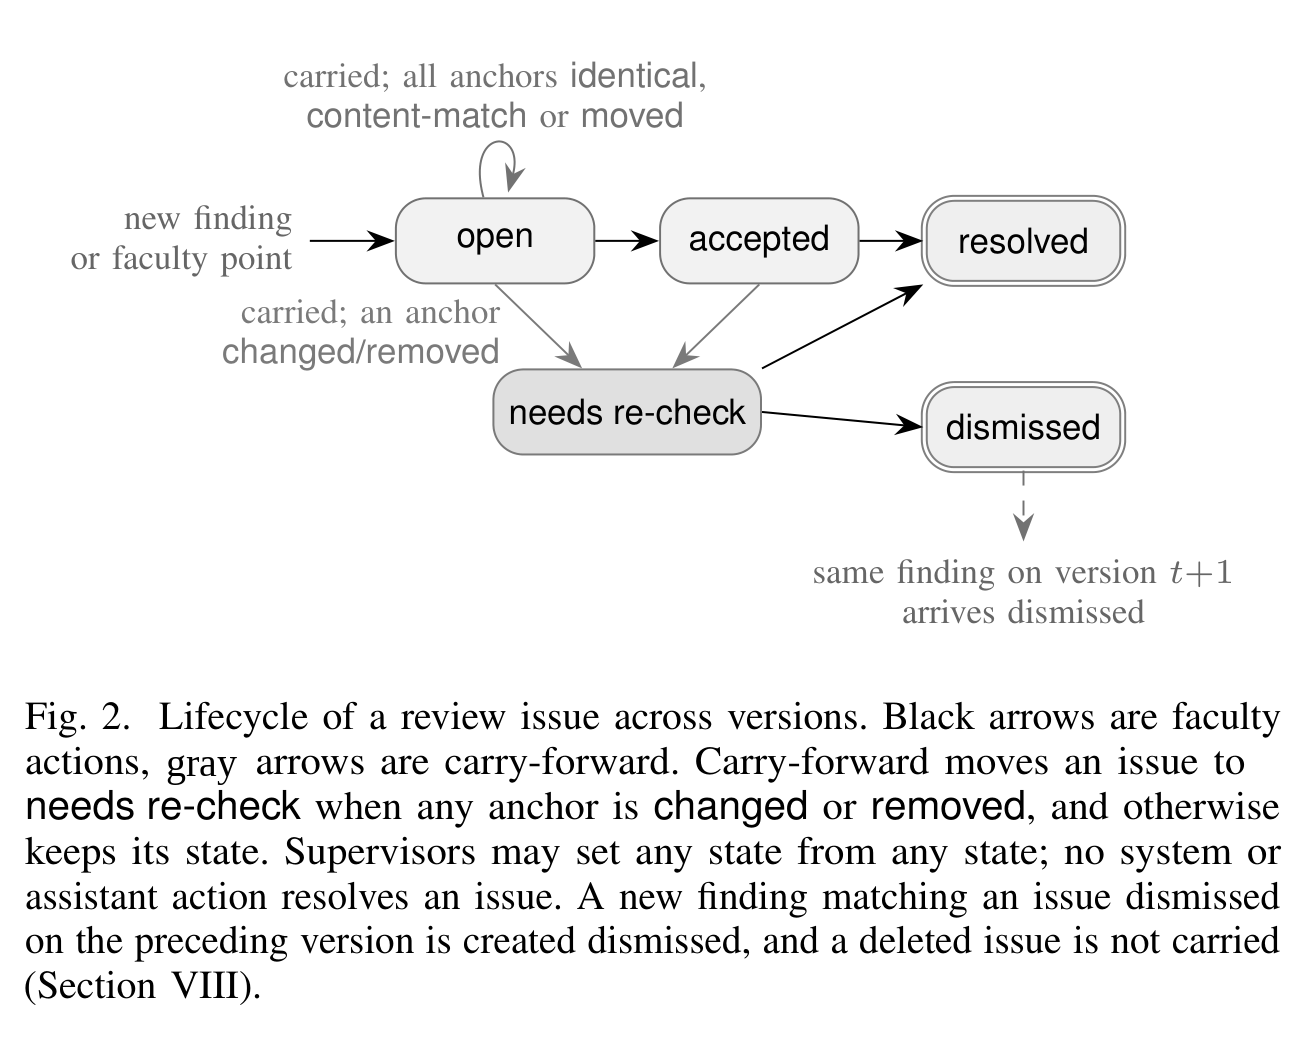
\includegraphics[width=\columnwidth]{assets/figure_2.png}
\end{figure}


If a finding has been raised again in analysis, it is matched with a carried forward issue, based on category, title and common evidence. Thus duplicate concerns in carried forwards are avoided. If a new finding matches any of those that were rejected in the previous version, based on category and the first 200 characters in Normalised form, then a finding will be made with the same status of being rejected. This heuristic is applied so that findings with similar opening paragraphs will be merged. However, if findings are reworded they can avoid matching (VIII). Notes added to carried issues (audio, video, image) are carried forward with the issue. Notes pinned to code are rediscovered in the cascade. The lifecycle is summarised in Figure 2.


\subsection{Three Properties and Five Safety Requirements}


Let $q_0$ denote the quotation of issue $i$, and $\rho_t(a)$ be the actual position of $a$ within $V_t$. (If the reviewed code does not exist, then $\rho_t(a)=\bot$.) We consider three properties. The first two properties are about code changes ($\delta_t(a)$ true means that code has changed from $q_0$ or that it does not exist), and correctness of anchoring ($w_t(a)=\rho_t(a)$). The third property, unresolved supervisor concerns, is only determined by supervisor actions. Changes outside quoted lines will not satisfy $\delta_t(a)$.


Given a re-check $r_t(a)$ on issue $i$ with issue state $\sigma_t(i)$, the required properties are:


\begin{itemize}
\item \textbf{S1:} $\delta_t(a)\Rightarrow r_t(a)$ (Modified targets must request a re-check).
\item \textbf{S2:} $w_t(a)\notin\{\bot,\rho_t(a)\}\Rightarrow r_t(a)$ (Incorrect positions must raise re-checks).
\item \textbf{S3:} $w_t(a)=\bot\Rightarrow r_t(a)$ (Missing targets must raise re-checks).
\item \textbf{S4:} Transitions to \emph{resolved} or \emph{dismissed} status must be made by supervisors.
\item \textbf{S5:} If an issue is not closed by a supervisor then it will remain active in $V_{t+1}$. If S1 is satisfied by an anchor then a re-check must be requested.
\end{itemize}
An anchor may be correctly placed (\emph{verified}), incorrectly placed (\emph{ambiguous}), or \emph{missing}. The property of being correctly placed is conditional. The assumptions of S1 require that the returned window contains the correct code, or none at all. That is, there should be no hiding of meaningful changes during normalisation. S2 requires that incorrect windows contain different code to the original quote. If lines are duplicated identically, or moved with meaningful indentation, these assumptions are violated (see Table~III). S3 results from the rules for requesting re-checks. S4 and S5 are checked using transitions in the application’s issue states given in Section VIII. In particular, identical duplicates in adjacent lines could be returned without a re-check, and edits to control flow surrounding unmodified quoted lines do not fall under the definition of changes to quoted spans. Therefore while the guards ensure that fewer failures are observed, we cannot guarantee that all meaningful changes will be detected. Even if a re-check is requested due to correct placement, we cannot be certain that the underlying concern has been resolved.


\section{System Architecture}


Living Review operates as part of a larger review composing system in the capstone review portal (see deployment diagram in extended report.) Caddy serves the client, and routes requests to a FastAPI server which manages user authentication, authorisation for all secure endpoints, data validation, and persistent data. Rule checking, language model, and partner-based trace (with signed results) of submitted code are performed by workers within a Celery queue and reviews composed. Version, issue, anchor, revision and change-log data is stored in PostgreSQL. Archives and media notes are stored in a store, using SHA-256 hash values as keys. Data. Review versions form a linear history. Each version contains exactly one review document. This review contains multiple issues identified by supervisors, each with status, severity, category, title, body and up to 12 anchors. The reference to the issue’s origin, given by carry:vt:id ensures idempotency in composing. Any editing of a version adds an attributed revision, and must be based upon a previous revision. This allows detection of parallel editing. When a review is composed, the version’s row is locked to allow for parallel composing by multiple clients. Issues are carried forward before running new analysis, to ensure any repeated findings match existing issues. The review page includes banners for how many issues have been carried forward (N) and require rechecking (M). Issues carried forward include a tag with “From version n”. Anchors include a note in plain text. If an assistant is used, review points can be edited using undoable tool calls in journaled revisions. It is recommended to resolve or dismiss a point, but this will only take effect if applied by a supervisor. Evaluated functions were run on a fixed snapshot of source code (as given in the artifact). Guarding and identity rules were evaluated on this snapshot, and have not yet been included in the deployed implementation.






\begin{table*}[!t]
\caption{Safety Failure Mechanisms}\label{tab:failure-mechanisms}
\centering\footnotesize
\setlength{\tabcolsep}{3pt}
\begin{tabular}{@{}L{.13\textwidth}L{.07\textwidth}L{.37\textwidth}L{.14\textwidth}L{.24\textwidth}@{}}\toprule
Mechanism & Breaks & Minimal counterexample ($V_0\rightarrow V_t$) & Addressed by & Residual \\ \midrule
Identical copy & S1, S2 (A3) & \texttt{a.py} and \texttt{b.py} hold the same retry loop; the reviewed loop in \texttt{a.py} is edited, and the unchanged copy in \texttt{b.py} is returned as \lbl{moved} & copy guard (AG, AGi) & copies adjacent to the original or added by the same revision (Section~VII-E); the guard asks but does not find the reviewed copy \\
Hidden indentation & S1 (A2) & \texttt{if ok:} / \texttt{\ \ send()} becomes \texttt{send()} at the outer level; stripped text is equal, so \lbl{content-match} & IG & a layout signal, not equivalence; relative only outside Python \\
Wrong fuzzy hop & S1 (A1) over versions & a look-alike window is accepted as \lbl{changed} at hop 3, carry replaces the quotation, and later hops compare against the wrong text & identity rule & choice of floor; some placements become lost \\
Locator verdict & S1 & a language model reports a region unchanged although its quoted lines were edited & labels from $q_0$ & none for S1; placement stays the locator's \\
Insertion around the quotation & none: outside $\delta$ & a suggestion wraps the reviewed call in a new guard clause; the quoted lines stand verbatim, so no label changes (Section~VII-D) & partly AG & a check of the lines around the span \\
Deleted target placed on look-alike & validity only & the reviewed block is deleted and a similar block nearby passes $\theta$; the request fires but points at other code & none & a misdirected request \\
Issue deletion & S5 & a supervisor or the assistant deletes an active issue; it is not carried & stronger contract (Sec.~VIII) & implemented: journaled undo only \\
Dismissal key collision & S4, S5 & a different finding with the same first 200 characters arrives \lbl{dismissed} & stronger contract & implemented: heuristic key \\
Uncomposed version & S5 & $V_2$ is never composed, so $V_3$ receives none of $V_1$'s issues & stronger contract & implemented: needs recomposition \\ \bottomrule
\end{tabular}
\end{table*}

\section{Evaluation Method}
\subsection{Retained Data and Excluded Repository Collections}
Observations were not merged, but kept separate. \textbf{Controlled experiments} were applied to 117 Python files (32,446 lines) using 12 edit types, with 300 experiments per type, giving 3,600 observations (primary seed). A separate replication seed was used. Edit types indicate expected location and edit labels. These edits are artificial, and the occurrence probability of errors occurring naturally could not be estimated. The controlled source code was taken from implementation and tracing code. The 117 files were not strictly public sources. This does not form a benchmark of independent public code that can be reproduced. The edited output data are just validation tools. The constructed stress and copy suites also use implementation-derived source files; they are not independent public-code benchmarks. If the evaluation was entirely without author owned code, the experiments would need to be performed on frozen public files, and re-run.

\textbf{Public Python histories:} Requests, Flask, Click, HTTPX, and Rich. Using the first parent commit history for these, 3,156 source commits were produced. Two samples of different types were taken. A uniformly sampled sample was taken (8,805 observations), and one targeted for edits (2,454 observations), giving 11,259 total observations. Code was not executed. In the case of public source code, the number of observations in each sample can be inferred from the macro data in the source code. Hence, unlike the aggregate of public and internal code, this data does not combine public and internal code. Uniform and targeted samples are given separately as the distribution of classes in each sample differs considerably.

\textbf{External Sources, Public.} CodeMapper benchmark \cite{codemapper2026} – 200 manually annotated regions, 2,392 external regions. GitHub review suggestion data – sample of 998 suggestions from Python, Typescript, Go, Rust and Java. \textbf{Author-derived tests.} Artificial stress test data with 23,550 cases to test indentation, duplication, very short anchor points and compound edits. Parametric copy data – 6,800 existing copies and 800 same version copies. These data sets have different reference definitions and cannot be combined with natural source code data.

\textbf{Exclusions.} 4 private project commit histories and 20 student repositories selected by the authors from public sources. No results were calculated purely from these sets. Grouped statistics were not given for the 9 projects, nor were 10-commit simulations of mixed populations. Totals were also excluded from public source code where the breakdown was not separately archived, to ensure that these totals do not represent purely public data.

\begin{table}[!t]
\caption{Retained Evaluation Populations}
\label{tab:populations}
\centering\footnotesize\setlength{\tabcolsep}{3.4pt}
\begin{tabularx}{\columnwidth}{>{\raggedright\arraybackslash}p{.37\columnwidth}X}
\hline
Population & Reference and size \\
\hline
Controlled edit seed (author-derived) & 3,600 synthetic trials; 12 operators; replication seed \\
Five public Python histories & 8,805 uniform + 2,454 edit-targeted observations \\
CodeMapper external benchmark & 200 independently human-annotated regions; 2,392 in full external set \\
Constructed stress cases (author-derived) & 23,550 generated cases \\
Applied GitHub review suggestions & 998 suggestions; 10 repositories; 5 languages \\
Parametric copy suite (author-derived) & 6,800 existing-copy + 800 same-revision-copy trials \\
\hline
\end{tabularx}
\end{table}

\subsection{Reference Labels and Their Limits}
Functions were annotated using qualified names. Statement trees were synchronised using normalised tree structures. Locations were determined based on matching statement trees. Some substitutions could be performed by matching the types of elements. If a unique matched tree is found then alternative locations can be searched. Observations that were ambiguous were removed according to the initial annotation protocol. This is purely a \emph{syntactic annotation} and does not represent knowledge on real execution behaviour or concerns of supervisors. The independently annotated CodeMapper regions and review suggestion oracle provide additional evidence with different uncertainties. In a multi-stage code review benchmark, defectiveness between stages is explicitly tested \cite{mcrbench2026}. These tasks are outside of this investigation, but do give motivation for future independent longitudinal testing. However, the total number of blinded adjudications by models in previously published results (in both public and private data) are not included in this edition. For these totals, there was no public-only group defined.

\subsection{Locators and Baselines}
The cascade has three static, line differential, or near match strategies. For this cascade, we evaluate static matches, normalised intra-file matches, fuzzy local matches and inter-file matches. The cascade has been implemented previously with a different ordering of tiers, and different thresholds. Alternative implementations exist including a context sensitive line matcher derived from LHDiff \cite{lhdiff2013}, CodeMapper \cite{codemapper2026}, GumTree \cite{gumtree2014} (based on syntactic tree differences) and two language model driven remote matchers. The safety tier derives change classification from the original reviewed match. Indentation and copy checks are performed without altering the location of the returned window. If the variable height matching configuration is used, then the position of the cascade may be altered.

\subsection{Outcome Definitions and Statistics}
Let C be the set of anchors with edited/deleted code in review. Let P be anchors with preserved quote content, S be surviving anchors, and A be all anchors. Let R be requested reviews. False omission rate is given by $|\{c\in C:\ell(c)\notin R\}|/|C|$. False positive rate is given by $|\{p\in P:\ell(p)\in R\}|/|P|$. Silent error rate is given by $|\{a\in A:\text{wrong window and }\ell(a)\notin R\}|/|A|$. Target misdirection occurs if a target is misplaced incorrectly, i.e. the review is requested but the target is incorrect. Lost anchors occur if an anchor survives, but no location is returned. Correct placement and classification is also shown. In the public results only, counts in numerators and denominators were taken from archived results. For retained benchmark and stress results, original fixed protocols were used. This is conservative in separating data sets as previously published evidence has shown that performance of automatic review is highly dependent on curating data sets and experimental protocols \cite{tufano2024,pirouzkhah2026}. For the edit-targeted public sample, $|A|=2,454$, $|C|=1,930$, $|P|=524$ and $|S|=2,359$. For the uniformly sampled public data, these are 8,805, 161, 8,644 and 8,786 respectively. For the independent human-annotated benchmark, they are 200, 130, 70 and 156. No new confidence intervals or significance tests have been drawn from previous pooled results (public and private).

\subsection{Evidence Strength and Exposure}
\begin{table}[!t]
\caption{Strength of Evidence}
\label{tab:evidence-tiers}
\centering\footnotesize\setlength{\tabcolsep}{3pt}
\begin{tabularx}{\columnwidth}{>{\raggedright\arraybackslash}p{.26\columnwidth}X}
\hline
Evidence & Appropriate inference \\
\hline
Synthetic controlled tests & Mechanism checks, not natural prevalence \\
Five public histories & Retrospective, syntactic-reference performance; public-only strata \\
External human benchmark & Placement against independent human annotations \\
Applied suggestions & Application-derived, rule-classified change proxy \\
Held-out constructed stress & Failure modes under deliberately selected conditions \\
Hosted tools and models & Dated, partly nondeterministic observations \\
\hline
\end{tabularx}
\end{table}

Because the safety mechanisms and thresholds were designed using real data, these analyses are retrospective. Although public data was used, non-deterministic tool accuracy from CodeMapper means that the resulting data from different runs cannot be treated as precise ground truth. Macro provenance information for the baseline (public only) can be found in the referenced artefact.

\section{RQ1: Where Is the Anchored Code Now?}
\textbf{Controlled edits.} In the 3,600 trials, the cascade achieved 98.5\% accuracy in locating edits (compared to 74.9\%, 58.3\%, and 41.7\% for exact quotes, drift diffs, and fixed lines respectively). Of the 3,000 anchors remaining after edits, 2,965 (98.8\%) were located accurately. These statistics reflect uniform weighting in the design of this operation, rather than the distribution of edits in real code.

\textbf{Real data (excluding excluded repos).} In the edit targeted stratified sample ($n=2,454$), the cascade achieved 66.8\% (1,639/2,454) correct placement or correct absence, among all 2,454 anchors. It achieved 72.5\% accuracy in deciding whether or not there was change, and placed 65.8\% of remaining targets accurately. The contextual tracker achieved 83.6\% in both. However, the previous version of the cascade achieved 74.3\% accuracy overall. By adjusting the cascade threshold, the accuracy of placing anchors in this stratified sample improved to 83.7\% (from 65.8\%). This resulted in fewer anchors being lost (reduced from 27.8\% to 1.4\%), but resulted in more misplaced re-check requests (increased from 5.7\% to 15.6\%) (see Table~VI). This result is not prospectively selected. In the uniformly sampled public stratified sample ($n=8,805$), a much higher accuracy was achieved (99.4\%). As such, this stratified sample cannot be said to have a general accuracy.

\begin{table*}[!t]
\caption{Public Python History Outcomes}
\label{tab:public-only-baselines}
\centering\scriptsize\setlength{\tabcolsep}{3.6pt}
\renewcommand{\arraystretch}{1.18}
\begin{tabular}{lrrrrrrrr}
\hline
Method & Correct & Class & Place & Miss & Silent & Misdir & Lost & Extra \\
\hline
\multicolumn{9}{l}{\emph{Edit-targeted public histories ($n=2,454$)}}\\
Cascade, deployed & 66.8 & 72.5 & 65.8 & 0.9 & 0.8 & 5.7 & 27.8 & 0.0 \\
Cascade, earlier version & 74.3 & 86.3 & 74.4 & 1.1 & 1.0 & 12.8 & 12.4 & 0.0 \\
Cascade, calibrated threshold & 82.6 & 96.5 & 83.7 & 0.5 & 0.5 & 15.6 & 1.4 & 1.1 \\
Contextual tracker & 83.6 & 85.6 & 83.6 & 0.3 & 0.2 & 2.6 & 11.6 & 13.7 \\
Exact quotation & 22.8 & 22.8 & 19.9 & 0.5 & 0.4 & 0.0 & 79.9 & 10.3 \\
Diff drift & 21.2 & 21.2 & 18.0 & 0.0 & 0.0 & 0.0 & 82.0 & 18.9 \\
Fixed line & 11.5 & 11.5 & 7.9 & 0.0 & 0.0 & 0.0 & 92.1 & 64.3 \\
\hline
\multicolumn{9}{l}{\emph{Uniformly sampled public histories ($n=8,805$)}}\\
Cascade, deployed & 99.4 & 99.5 & 99.4 & 1.9 & 0.0 & 0.1 & 0.5 & 0.0 \\
Cascade, earlier version & 99.6 & 99.7 & 99.6 & 1.9 & 0.0 & 0.2 & 0.2 & 0.0 \\
Cascade, calibrated threshold & 99.7 & 99.9 & 99.7 & 0.6 & 0.0 & 0.3 & 0.0 & 0.0 \\
Contextual tracker & 98.7 & 98.7 & 98.7 & 0.6 & 0.0 & 0.0 & 0.3 & 1.0 \\
Exact quotation & 98.2 & 98.2 & 98.2 & 0.6 & 0.0 & 0.0 & 1.8 & 0.2 \\
\hline
\end{tabular}
\parbox{.98\textwidth}{\footnotesize Percentages; metrics have different denominators. \emph{Correct}: correct location or correct absence among all targets; \emph{Class}: accuracy of change classification; \emph{Place}: correct location among surviving targets; \emph{Miss}: edited/deleted anchors without re-check; \emph{Silent}: wrong location without request; \emph{Misdir}: wrong location with request; \emph{Lost}: surviving targets without a location; \emph{Extra}: unnecessary request on preserved content. For the deployed edit-targeted cascade, \emph{Correct} is 1,639/2,454 (66.8\%), \emph{Class} is 1,779/2,454 (72.5\%), and \emph{Miss} is 17/1,930 (0.9\%). Calibration reduces \emph{Lost} from 27.8\% to 1.4\% but raises \emph{Misdir} from 5.7\% to 15.6\%. Reconstructed solely from the archived \texttt{smPubTgt} and \texttt{smPubUni} numerator/denominator macros; this is not a new experiment.}
\end{table*}

\textbf{Independent CodeMapper Benchmark.} See Table~VII. In 200 manually labelled benchmark regions, the cascade achieved 66.0\% accuracy in determining if an anchor started at the correct line (or did not exist in the file). The contextual tracker achieved 85.5\% accuracy, and CodeMapper achieved 91.5\% \cite{codemapper2026}. CodeMapper achieved 74.0\% accuracy in locating exact character regions compared to 24.5\% achieved by the deployed cascade. The full external benchmark contains 2,392 regions. Tool annotated regions have been separated from manually annotated regions. Therefore, 91.5\% accuracy equates to 183/200. In Table~IX, CodeMapper was run separately. Additionally, in determining accuracy, the 44 regions where an anchor did not exist have been removed from the denominator. Therefore, 93.6\% equates to 146/156 correctly located remaining anchors. These results do not conflict. Using the independent benchmark allows for a more stringent, although higher, comparison of accurate placing within benchmarks than the syntax-based, publicly available labels.

\begin{table}[!t]\caption{Independent Region Benchmark}\label{tab:human}
\centering\footnotesize\setlength{\tabcolsep}{2.5pt}
\begin{tabular}{@{}lrrrrrr@{}}\toprule
 & \multicolumn{4}{c}{Human A/B (200)} & Non-Py & All \\ \cmidrule(lr){2-5}
Method & Line & Chars & Missed & Silent & Line & Line \\ \midrule
Deployed cascade & 66.0 & 24.5 & 8.5 & 3.5 & 63.7 & 57.5 \\
All guards, $\theta=.85$ & 70.0 & 26.0 & 1.5 & 0.5 & 67.8 & 64.5 \\
All guards, $\theta=.55$ & 77.0 & 17.5 & 1.5 & 0.5 & 77.4 & 70.9 \\
Cascade v1 & 70.0 & 21.5 & 8.5 & 3.5 & 67.1 & 59.5 \\
Contextual tracker & 85.5 & 28.0 & 3.8 & 0.0 & 86.3 & 70.2 \\
GumTree & 62.0 & 17.0 & 1.5 & 0.5 & 71.2 & 66.8 \\
CodeMapper & 91.5 & 74.0 & 4.6 & 1.0 & 89.7 & 86.2 \\
\bottomrule
\end{tabular}
\tablenote{Percentages. Line: file and start line, including correct absence. Chars: exact character region. All guards: IG, the original copy guard AG and VW (Table~IX uses the corrected AGi). CodeMapper: this evaluation's run and change adapter (Table~IX uses a later run with the cascade's quotation labels). Non-Py: the 146 human-annotated regions outside Python. All: all 2,392 external regions, including tool-derived Java histories. Living Review sees only the paired files. GumTree execution failures count as incorrect. The pinned CodeMapper is not fully deterministic (Section~V-E).}
\end{table}

\textbf{RQ1 Answer.} The deployed cascade does not perform best in locating anchors. Within publicly available Python edit targeted data, locating anchors with the contextual tracker performs better. CodeMapper performs significantly better in this independent benchmark. As such, the safety layer can be considered as an effective policy to apply to stronger location techniques. It cannot be assumed that the original cascade is universally optimal.

\section{RQ2: Does the Safety Layer Keep Changed Code in Front of the Supervisor?}
\subsection{Failure Mechanisms and Constructed Stress}
Within public Python projects, 17 of the 1,930 (0.9\%) modification/deletion targets were not requested to be re-reviewed by the cascade, and 20 of 2,454 (0.8\%) were silently misplaced (without a re-check request). Within uniform projects, 3 of 161 (modification/deletion) targets were not requested to be re-reviewed. These numbers are only within public projects, and do not include the data from the previous 9-project aggregation. Exact duplicates, normalised whitespace, similar fuzzy duplicates and multi-revision re-anchoring are distinct failure types. Examples of these failure scenarios are given in Table~III.

Stressed scenarios: The stressed scenarios deliberately increase these failure scenarios. The cascade failed to trigger re-reviews for all 1,200 behaviour changing indentation changes in Python. However, adding indentation and duplicate guards, with variable window sizes, removes this error within this suite. However, extra re-review requests arose in layout-only cases. In duplicate suites, unchanged duplicates can be confused with code under review. Duplicate guards often make this uncertainty apparent rather than resolving it in the wrong location. These rates are stresses, and are not estimates of prevalence in the population.

\begin{table*}[!t]
\caption{Safety Guard Stress Tests}
\label{tab:guard-stress}
\centering\footnotesize\setlength{\tabcolsep}{4.3pt}
\renewcommand{\arraystretch}{1.12}
\begin{tabular}{lrrrrrr}
\hline
Method & \multicolumn{3}{c}{Indentation} & \multicolumn{3}{c}{Duplicate copies} \\
 & Miss & Silent & Extra & Miss & Silent & Extra \\
\hline
Cascade baseline & 100.0 & 0.0 & 0.0 & 89.7 & 69.1 & 0.1 \\
Cascade + AG & 100.0 & 0.0 & 0.0 & 21.9 & 27.4 & 27.7 \\
Cascade + AGi & 100.0 & 0.0 & 0.0 & 29.2 & 32.4 & 24.4 \\
Cascade + AG2 & 100.0 & 0.0 & 0.0 & 89.4 & 66.6 & 0.4 \\
Cascade + IG+AGi+VW & 0.0 & 0.0 & 25.0 & 29.2 & 32.3 & 24.6 \\
CodeMapper + labels & 85.0 & 0.0 & 3.3 & 46.1 & 43.8 & 10.8 \\
CodeMapper + IG & 0.0 & 0.0 & 26.9 & 46.1 & 43.8 & 10.8 \\
CodeMapper + AG & 85.0 & 0.0 & 3.3 & 11.9 & 18.6 & 36.4 \\
CodeMapper + AGi & 85.0 & 0.0 & 3.3 & 18.5 & 23.2 & 33.1 \\
CodeMapper + IG+AGi & 0.0 & 0.0 & 26.9 & 18.5 & 23.2 & 33.1 \\
\hline
\end{tabular}
\par\vspace{6pt}
\begin{tabular}{lrrrrrr}
\hline
Method & \multicolumn{3}{c}{Short anchors} & \multicolumn{3}{c}{Compound edits} \\
 & Miss & Silent & Extra & Miss & Silent & Extra \\
\hline
Cascade baseline & 71.0 & 37.9 & 0.2 & 1.1 & 0.2 & 28.9 \\
Cascade + AG & 0.1 & 0.1 & 21.6 & 0.6 & 0.0 & 60.9 \\
Cascade + AGi & 0.1 & 0.1 & 21.5 & 0.6 & 0.0 & 45.8 \\
Cascade + AG2 & 0.0 & 0.0 & 17.3 & 1.0 & 0.0 & 29.1 \\
Cascade + IG+AGi+VW & 0.0 & 0.0 & 34.1 & 0.0 & 0.0 & 66.7 \\
CodeMapper + labels & 0.0 & 0.0 & 13.5 & 0.4 & 0.0 & 57.5 \\
CodeMapper + IG & 0.0 & 0.0 & 26.0 & 0.1 & 0.0 & 69.7 \\
CodeMapper + AG & 0.0 & 0.0 & 25.1 & 0.0 & 0.0 & 89.3 \\
CodeMapper + AGi & 0.0 & 0.0 & 25.0 & 0.0 & 0.0 & 74.1 \\
CodeMapper + IG+AGi & 0.0 & 0.0 & 37.5 & 0.0 & 0.0 & 75.9 \\
\hline
\end{tabular}
\parbox{.96\textwidth}{\footnotesize Percentages on a fixed, constructed seed: indentation (1,200 changed / 1,200 preserved), duplicate copies (1,500/2,250), short anchors (5,400/10,800), and compound edits (798/402). Miss is over changed/deleted cases, Extra over preserved cases, and Silent over all cases. AG, AGi and AG2 are distinct copy guards; IG is the indentation guard and VW the variable-height window. The suites use implementation-derived source files, intentionally overrepresent failure mechanisms and are not prevalence estimates.}
\end{table*}

\subsection{Safety Layer with Independent References}
Only the remaining \emph{independent manually annotated} and \emph{synthetic stressed} columns from the original by-layer comparison are included in Table~IX. Other columns were either aggregated from internal/public histories or taken from the deleted student repository collection. The guards do not alter the window generated by CodeMapper or the contextual tracker, but raise a request to the supervisor if any doubts occur regarding the quotation or context. Additionally, the height of the cascade may vary.

\begin{table*}[!t]
\caption{Safety-Layer Outcomes}
\label{tab:retained-guards}
\centering\footnotesize\setlength{\tabcolsep}{4.5pt}
\begin{tabular}{lrrrrrr|rrrrrr}
\hline
& \multicolumn{6}{c|}{Human-annotated regions ($n=200$)} & \multicolumn{6}{c}{Constructed stress cases ($n=23,550$)} \\
Method & Place & Miss & Silent & Misdir & Lost & Extra & Place & Miss & Silent & Misdir & Lost & Extra \\
\hline
Cascade, deployed & 62.2 & 8.5 & 3.5 & 9.0 & 27.6 & 34.3 & 66.0 & 71.8 & 37.1 & 0.9 & 3.3 & 0.9 \\
Cascade + IG + AGi + VW & 67.3 & 3.8 & 0.5 & 9.0 & 26.3 & 44.3 & 69.7 & 4.9 & 5.2 & 29.9 & 3.0 & 32.8 \\
CodeMapper + labels & 93.6 & 3.1 & 0.0 & 7.5 & 1.3 & 35.7 & 83.0 & 19.3 & 7.0 & 4.6 & 10.6 & 13.4 \\
CodeMapper + IG + AGi & 93.6 & 2.3 & 0.0 & 7.5 & 1.3 & 44.3 & 83.0 & 3.1 & 3.7 & 7.9 & 10.6 & 37.0 \\
Contextual tracker + labels & 82.7 & 3.8 & 0.0 & 3.0 & 14.7 & 35.7 & 82.0 & 22.0 & 7.7 & 0.1 & 11.8 & 13.2 \\
Contextual tracker + IG + AGi & 82.7 & 3.1 & 0.0 & 3.0 & 14.7 & 44.3 & 82.0 & 3.3 & 4.1 & 3.7 & 11.8 & 37.9 \\
\hline
\end{tabular}
\parbox{.97\textwidth}{\footnotesize From the retained human-annotated and constructed stress populations; no private or student-selected observations are included. Place: correct location among surviving targets; Miss: changed/deleted without a re-check; Silent: wrong placement without a request; Misdir: wrong placement with a request; Lost: surviving target without a location; Extra: request when content is preserved. Rates have distinct denominators; in the human benchmark Place excludes 44 absent targets (CodeMapper 146/156=93.6\%), whereas Table VII includes correct absence over all 200 (183/200=91.5\%). The measurements also use distinct runs of a partly nondeterministic CodeMapper build. Label-only versus guarded miss: 4/130 versus 3/130; extra: 25/70 versus 31/70.}
\end{table*}

On the synthetically stressed data, adding indentation and copy guards to the CodeMapper layer decreased missed checks from 19.3\% (only quotation labels) to 3.1\%, but increased unnecessary checks from 13.4\% to 37.0\%. On the manually annotated independent sample, missed checks were reduced from 4/130 (3.1\%) to 3/130 (2.3\%) and unnecessary checks increased from 25/70 (35.7\%) to 31/70 (44.3\%). This improvement in avoiding just one missed check in 130 modified/deleted anchors does not indicate a great overall improvement. Neither decrease in workload can be confirmed as we did not observe actual costs for the supervisors. A natural history with only public guards is not shown here as in the archive comparison table, in-house and public histories have been aggregated. This would require a filtered replay to be performed separately.

\subsection{Language Models and Change Labels}
Beam 1.0 failed to flag 41 of 1,930 required changes and Nemotron 3.5 Super failed to flag 12. Using the quote and guards reduced the number of missed changes in this instance to 0 (note: results were generated by the hosted models at a point in time and therefore should not be viewed as deterministic). However, some missed changes remained in the manually annotated subset. Therefore, decisions on whether a concern has been adequately addressed are not automatically decided using language model output. An advisory annotation may be given.

\subsection{An Independent Multi-Language Suggestion Oracle}
Review suggestions are presented with quoted and suggested code. Within pull request heads, we can infer whether they were applied, unchanged, modified, removed, or ambiguous. The dataset comprises 998 suggestions from 486 merged pull requests across 10 public repositories. 2 repositories from each of Python, TypeScript, Go, Rust, and Java. There are 361 applied, 189 unchanged, 336 modified, 38 removed and 74 ambiguous suggestions. Both independent classification methods agreed on labels. However, applying a suggestion does not necessarily imply that the concern has been addressed.

For applied or unchanged targets, CodeMapper had an accuracy of 91.1\% compared to 78.9\% with the implemented cascade and 36.7\% using GitHub’s current position policy. (See Table~X). We observe that the quotation may hide changes at line level. If only quotation changes are considered, then changes like comparisons: a suggestion can be applied by inserting a guard will be missed in unchanged quoted code. This indicates we should continue to maintain supervision to ensure concerns are resolved even if quoted code appears unchanged.

\begin{table}[!t]\caption{Review Suggestion Oracle}\label{tab:suggestions}
\centering\footnotesize
\setlength{\tabcolsep}{3pt}
\begin{tabular}{@{}lrrrrrr@{}}\toprule
Method & Place & Miss & Silent & Misdir & Lost & Extra \\ \midrule
GitHub outdating & 36.7 & 16.2 & 3.2 & 0.0 & 59.8 & 12.2 \\
Cascade, deployed & 78.9 & 3.1 & 0.0 & 2.2 & 19.5 & 0.0 \\
Cascade+IG+AGi+VW & 80.5 & 3.1 & 0.0 & 1.9 & 18.2 & 4.2 \\
CodeMapper+quote & 91.1 & 2.7 & 0.0 & 5.1 & 5.6 & 4.2 \\
\quad +IG+AG & 91.1 & 1.1 & 0.0 & 5.1 & 5.6 & 9.5 \\
\quad +IG+AGi & 91.1 & 2.7 & 0.0 & 5.1 & 5.6 & 5.8 \\
\bottomrule
\end{tabular}
\tablenote{998 review suggestions from 10 repositories in 5 languages; scope is the file pair. Place and Lost: over the 550 applied or untouched targets (applied: start inside the suggested text). Miss: over the 735 changed targets (applied, rewritten, deleted). Extra: over the 189 untouched targets. Silent and Misdir: over all 588 scored targets. GitHub: the thread's current outdated flag. Ambiguous targets (74) are not scored.}
\end{table}

We include results from running the concern-level language model on the suggestion sample as exploratory comparison. Although applied suggestions may indicate that a comment was addressed more frequently than quotation change, it cannot be inferred that the substantive concern has been resolved. While predictions may be used to prioritise reviews, issues cannot be closed based on them.

\subsection{Copy Distance and Multiplicity}
This category of parametric variation changes the number of copies, and their location. It also specifies if the base is modified, removed, moved or left. The 116 source files in this category come from the same derived Python corpus as the controlled edits. As these instances have been manually created, they cannot be considered to be a fully public-sourced reproduction until they are re-created on public code. However, 6,800 instances (plus 800 instances with identical revisions) have been created (Table~XI). Without appropriate guards in the copy intensive variations, 82.1\% of checks failed (compared to 8.5\% with the corrected guard). Some errors resulted in queries being made to the incorrect copy. If an adjacent copy exists on the same line as the base, then even checking for unexpected locations will fail. Similarly, if there is a copy in the same revision as modification to the base, there is no reliable origin signal. This is not due to whether the source repository is a student project, but due to indistinguishable data.

\begin{table*}[!t]
\caption{Identical-Copy Stress Tests}
\label{tab:copy-tests}
\centering\footnotesize\setlength{\tabcolsep}{5.0pt}
\renewcommand{\arraystretch}{1.15}
\begin{tabular}{lrrrrrr}
\hline
Method & Place & Miss & Silent & Misdir & Lost & Extra \\
\hline
Cascade baseline & 73.9 & 82.1 & 42.9 & 0.2 & 0.0 & 0.0 \\
Cascade + IG+AG+VW & 73.9 & 8.5 & 4.2 & 38.9 & 0.0 & 50.0 \\
Cascade + IG+AGi+VW & 76.5 & 8.5 & 4.2 & 37.0 & 0.0 & 0.0 \\
CodeMapper + quotation & 100.0 & 4.1 & 2.1 & 1.6 & 0.0 & 0.0 \\
CodeMapper + IG+AG & 100.0 & 3.3 & 1.7 & 2.1 & 0.0 & 50.0 \\
CodeMapper + IG+AGi & 100.0 & 3.3 & 1.7 & 2.1 & 0.0 & 0.0 \\
\hline
\end{tabular}
\par\vspace{6pt}
\begin{tabular}{lrrrrrrr}
\hline
Method & Adjacent & $\leq$20 & $>$50 & Cross-file & Shift extra & Same-rev. miss & Issue miss \\
\hline
Cascade baseline & 100.0 & 100.0 & 100.0 & 48.8 & 0.0 & 87.2 & 74.4 \\
Cascade + IG+AG+VW & 36.0 & 0.0 & 0.0 & 0.0 & 100.0 & 34.1 & 1.2 \\
Cascade + IG+AGi+VW & 36.0 & 0.0 & 0.0 & 0.0 & 0.0 & 40.1 & 2.5 \\
CodeMapper + quotation & 17.4 & 0.2 & 0.0 & 0.0 & 0.1 & 49.6 & 1.4 \\
CodeMapper + IG+AG & 14.1 & 0.0 & 0.0 & 0.0 & 100.0 & 21.5 & 0.5 \\
CodeMapper + IG+AGi & 14.1 & 0.0 & 0.0 & 0.0 & 0.1 & 26.5 & 1.1 \\
\hline
\end{tabular}
\parbox{.97\textwidth}{\footnotesize Six safety outcomes (upper panel) over 6,800 constructed trials drawn from 116 implementation-derived Python files. Lower panel: missed re-checks by nearest pre-existing copy distance (adjacent, within 20 lines, more than 50 lines, another file), unnecessary re-checks on shifted unchanged code, misses when the copy is added in the same revision (800 additional trials), and issue-level missed requests for 2,295 synthetic multi-anchor issues. These cases are constructed, not natural frequencies. The 116-file source set is not entirely public and requires substitution and rerunning for a strict public-input replication.}
\end{table*}

\subsection{Longitudinal Identity and Costs}
The identity rule means that the supervisor’s original quote $q_0$ remains unchanged. This avoids an erroneous intermediate match becoming a definitive reference in further versions. In the 10 commit replay results and supervisor intervention simulations, the totals for the public and internal project histories combined are not shown here. To find out whether this rule provides the same numerical benefits within only public histories, the filtered data would need to be re-run.

Safety layer, the number of additional requests increases in this layer. The benefit depends on the cost of incorrectly carrying forwards a change compared to making redundant confirmations. Within the independently annotated benchmark dataset and artificial stress test set, the increase in additional requests can be measured (Table~IX). However, no empirical weighting factors, review durations or realistic prevalence of issue changes could be found. As such, there is no universally optimal threshold or copy guarding policy which has been proposed.

\subsection{Answer to RQ2}
The results on the public subset (with manually annotated experiments) demonstrate the separation between moving code and resolving questions. While the quote markers and protec tion reduce the number of undetected changes (especially indents and copy-paste errors), they miss a proportion of misplaced windows. In addition, they can lead to more questions being raised with supervisors. It remains unclear how to deal with changes around constant quoted lines and identical similar copies. In order to generalise the rates found in previous experiments (with combined history) to the smaller dataset, it is important to run an experiment with only public data, with protection.

\section{RQ3: The Implemented State Contract}


Specification: A summary of the enforced transitions is given in the extended summary. There are thirteen enforced transitions (13 rows); these include the enforcer, transition between states, and implementation lines. It has been verified that no code path can result in resolved in the system. For faculty status, there are no preconditions, meaning that a supervisor can transition to any state from any state.


Static Analysis \& Bounded Model Checking: In static analysis, there were 26 calls to modify a review issue (create, update, delete, restore, undo). However, there were no direct assignments to the status. Therefore, no writer in the system can set an issue to resolved. Thus this claim relies on static analysis. In the bounded model checking of transitions for 2 findings and 2 versions, with non-deterministic labelling of movement for all carried issues, there were 7,179,369 states and 58,122,810 transitions. At depth 6, a resolved status was not reached in any system events (0 violations). Revision history was always append-only. Additionally, repeated composition had no effect. Issues could never be closed by the assistant without supervisor confirmation. However, one invariant was violated. Active issues were not moved to the next version in 629,056 transitions. This was due to deletion (314,528 deletions by the supervisor and 314,528 deletions by the assistant). Although deletion is reversible, once an issue has been deleted it will not be carried forward. Consequently, the verified claim is fairly limited. It has been verified that no systems events set an issue to resolved, however, it is possible that concerns no longer remain in the workflow. Testing scenarios: Of the scenarios testing review statuses and artifacts in the pinned application, 80 of 82 passed, 1 failed, and 1 was skipped (none due to review statuses). Eight scenarios were created to test submitting versions, importing signed analysis packages, and composing reviews via the interface. It was confirmed that: 3 versions had the correct labels applied (moved, modified, removed), modifying 1 supporting anchor resulted in a multi-anchor issue, composition was idempotent. Concurrent composition with PostgreSQL 17.10 resulted in no duplicates. Media notes were correctly linked to their issue/code. However, 3 were incorrect. The design was updated. When dismissing an issue, only the previous version is compared to using a heuristic key. Thus, if another finding has the same opening paragraph, it is suppressed. If a finding does not exist in a version, it appears open. Only the previous version is considered when moving issues forward, meaning that if a version has not been composed, it cannot be moved forward until it has been composed. If an unchanged file exceeds the carry size limit, it is labelled as removed in its anchor. This results in a false recheck rather than a silent error. Stronger Contract. Each gap in this property, what behaviour is actually seen, and suggested rules, are given in Table~XII. The invariants are stronger versions of S4 and S5. No resolved (S4a) or dismissed (S4b) status can be written by the system. Issues cannot be closed/withdrawn by the assistant without supervisor confirmation (S4c). Withdrawn issues are visible in later versions (S5-vis). When withdrawn by a supervisor, a visible tombstone remains for later versions to carry. The assistant can make only one proposal. Undoing reverses composition after withdrawal. Dismissal identity is defined by category, standardised title and a hash of reviewed quotations. This is compared to all previous versions. If a finding matches a dismissal, it is created open and includes a note detailing the dismissal. Thus, the system cannot dismiss an issue. If a version is late-composed, its descendants are recomposed. Gap Analysis: With two findings (conflicting keys), three versions, and all sixteen label combinations for two anchors, and all orderings of events for each gap to a depth of 8 (3455 and 3748 unique states), all gaps in the actual contract were reproduced with minimal event sequences. However, none of the gaps in the suggested contract were found. The suggested contract is specified and modelled, but not implemented; model checking does not establish deployed behavior. RQ3 Answer: No system events result in an issue being resolved.


\begin{table*}[!t]\caption{Review-State Contract}\label{tab:state-contract}
\centering\scriptsize\setlength{\tabcolsep}{2pt}
\begin{tabular}{@{}L{.16\textwidth}L{.27\textwidth}L{.31\textwidth}L{.11\textwidth}>{\raggedleft\arraybackslash}L{.045\textwidth}>{\raggedleft\arraybackslash}L{.045\textwidth}@{}}\toprule
Gap & Implemented & Proposed rule & Invariant & Impl. & Prop. \\ \midrule
Deletion (faculty) & Deleted item excluded from carry & Faculty withdrawal leaves visible tombstone & S5, S5-vis & 1 & 0 \\
Deletion (assistant) & Assistant deletion stops carry & Assistant proposal; faculty applies withdrawal & S4c, S5, S5-vis & 1 & 0 \\
Restoration across versions & Undo restores prior snapshot only & Recompose descendants after undo & Restoration, S5 & 1 & 0 \\
Dismissal key collision & Category plus first paragraph key conflates anchors & Category + normalized title + reviewed-quotation digest & Dismissal identity, S4b & 2 & 0 \\
Dismissal lapse after absent version & Only immediately previous version is checked & Compare dismissals across all earlier versions & Dismissal memory, S5 & 1 & 0 \\
Dismissed finding created closed by system & Matching new finding is created dismissed & Create open with prior-dismissal annotation & S4b & 1 & 0 \\
Uncomposed intermediate version & v3 reads only v2 and skips v1 issues & Compose latest ancestor; later v2 recomposes descendants & S5 & 1 & 0 \\
System write on closed issue (evidence replaced) & System replaces evidence and retains closed state & Evidence replacement never writes a closed state & S4a, S4b & 0 & 0 \\
\bottomrule
\end{tabular}
\end{table*}


However, the stronger property (S4 and S5 combined) is not satisfied within the implementation. Issues cannot be carried if deleted by supervisors/assistants, or if a version is not composed. Dismissal memory creates a new finding, which may have already been dismissed, and may result in a closing by the system. Within the suggested contract, these gaps have been filled. This contract should still be implemented within the portal.



\section{Threats to Validity}
\textbf{Construct Validity.} The validity of concerns, and therefore fixes, cannot be assumed based on edits. Suggestion reviews do not necessarily indicate correct fixes. Edits may alter program flow without changing anchor lines, and multiple identical copies may not provide enough information to identify original edits.

\textbf{Reference.} Five natural histories in Python were used. Pairs of same-type statements allow similar statements to be selected, and ambiguous cases were filtered out. Therefore results depend on decidability of references. An independently annotated subset of CodeMapper is available, though only 200 regions are included. Of the 998 suggestions in GitHub, they are externally written. The application category is not determined by human decision in this study. Both selected adjudication and localisation models from hosted models are not performed by humans.

\textbf{Selection bias.} Excluding 4 private histories, and 20 student-selected repositories reduces the range of coverage. This means we cannot assume the remaining 5 public projects form a representative sample of all software. Edits in controlled experiments and stress tests have selected failure modes overrepresented. Several safeguards were put in place following analysis of previous history results. As such they are retrospective. The independent benchmark, and out-of-sample generated cases provide complimentary rather than comparable evidence.

\textbf{Statistical bias.} Within the same repository and commit, target instances are not independent. Though counts of baseline for public-only cases retain independence, confidence intervals across combined cases, model adjudicated totals, 10-commit simulation rates, and comparisons between different configurations within each project, cannot be reasonably reused without recalculation. Similarly, some results from CodeMapper and language models are non-deterministic. Many secondary comparisons were exploratory; no new inferences are made in this edition using reduced corpus.

\textbf{External Validity.} All natural history commits used in Section VI come from 5 mature public Python projects. Suggestion oracle includes more languages, however it views pairs of files rather than longitudinal supervision. No supervisors or students were observed, and so this work does not quantify improvements in review time, feedback incorporation, learning, or workload.

\section{Discussion}
The results are presented for different comparison groups. For edit-targeted public Python histories, the basic model returns a correct location or correct absence for 66.8\% of anchors (1,639/2,454). Of the 1,930 edited/deleted targets, 0.9\% were not rechecked. The contextual model performs better on this group of examples, and CodeMapper performs better on the manually annotated 200 region benchmark. These comparisons vary in difficulty and quality of labelling. They should therefore be considered separate and no overall accuracy measure made.

Independent and stress tests demonstrate what improvements this layer makes. Using the same change labelling, indentation checks and copy checking outside the cascade, concern locations can be detected. However, we cannot claim to improve what window has been selected by the location model. We do transform some silent errors into explicit re-checks. This leads to more alerts for the reviewer, but it is unknown how this impacts learning, and the burden on the reviewer. In software review efficiency, review effort is treated as a constraint \cite{kudrjavets2024}. Therefore, when considering the impact of this work on a faculty member, the number of errors prevented and additional confirmations should be balanced, rather than maximising alerts.

Stable deployment settings mean that original quotations are maintained. Changes are labelled independently of location, if there are unclear or missing anchors these are made clear, and human intervention is required to resolve. The precise similarity threshold, and copy checking, must be decided for deployment. To determine these settings, a comparison using independent revision chains, and analysis of actual faculty decisions, must be performed. Future evaluation should consider both whether concerns are correctly located by faculty members, and whether appropriate feedback was given and followed. Therefore, usability of the system and student engagement should be considered separately from technical accuracy \cite{little2024,carlessyoung2025,weidlich2025}. None of the previously run evaluations for policy selection across 9 repositories, simulated supervision, or 10 commit trajectories (with public only outcomes) are reused in this work.

\textbf{Ethical Issues.} No private submissions from students were used in this evaluation. The natural history repositories and suggested changes from GitHub are public. However, in the controlled experimental setup and implementation logs there are restrictions on access, meaning that precise replication of these tests may not be possible. All model calls in this work were made using public code. If any further deployment studies were carried out authorisation and informed consent would be required.

\section{Conclusion}
This work considers changes in review concerns. A review concern can be raised if there is a change in quoted text (change evidence), the moved anchor is valid, and the supervisor decides to raise the concern. Five safety constraints have been defined. In cases where there is uncertainty either in code or resulting location, the layer adds a request for re-review. However, moving anchor points should never be sufficient for closing a concern.

Findings include synthetic controlled changes, five named public python repository history, independent benchmark in CodeMapper, structured stress testing and public GitHub suggested reviews. Findings from the public datasets indicate that the cascading system achieved 66.8\% correct location or correct absence among edit-targeted anchors (1,639/2,454), but achieved 72.5\% accuracy in determining the type of change in targeted code. Although calibration improved the number of surviving anchors, it increased the number of misplaced re-reviews. The independent benchmark indicates that CodeMapper performs better at placing review concerns. Stress test scenarios indicate that the guards provide safety, but require extra confirmation. Data from private histories and selected student repositories no longer contribute to findings. If just mixed denominator populations were present, findings are not reported. Data with only mixed population denominators are omitted (rather than re-labelled).

The application has another limitation. Deletion of code, incorrect matching, or absence of intermediate compositions may cause concerns to be lost from a review, despite a request to pay further attention to a concern. A strong issue state has been defined and modelled, but is not implemented in the current composition. The next steps are to re-run the guarded and longitudinal experiments using only preserved public data, implement the strong state, and evaluate supervisors on real, permission granted re-submissions. Currently, findings suggest technical safety mechanisms have been applied, but do not indicate improvements in educational outcomes.

\section*{Acknowledgment}
OpenAI Codex and Anthropic Claude Code were used widely during experimental design, benchmarking, analysis and reproducibility checks, and writing of parts of this paper. The research was directed by the authors. The scope of the findings and their interpretation was determined by the authors, and the authors are responsible for ensuring the accuracy and integrity of the final paper and supporting data.

\section*{Reproducibility}
\textbf{External Repositories Used.} Repositories used with natural data: Requests (\url{https://github.com/psf/requests}), Flask (\url{https://github.com/pallets/flask}), Click (\url{https://github.com/pallets/click}), HTTPX (\url{https://github.com/encode/httpx}) and Rich (\url{https://github.com/Textualize/rich}). Particular versions of these repositories, along with the numerator and denominator macros used to create public data, are available in the public artifact. Line History Code: \url{https://github.com/oselvar/lhdiff}. Region Mapping Code: \url{https://github.com/sola-st/CodeMapper}. Particular versions of GumTree and dependencies are provided in the artifact. Individually annotated regions come from the public benchmark provided by CodeMapper \cite{codemapper2026}.

\textbf{Reconstruction and Filtering.} The original mixed population data should not be considered as a source of the public only baseline data. Table~VI has now been updated to utilise existing count macros within \texttt{smPubUni} and \texttt{smPubTgt}, in \texttt{v12-ieee15/generated/numbers-v11.tex}. Targeted and uniform sampling have been separated in this update. Independent benchmarking tables and evaluation numbers maintain previously archived results. Synthetic suites contain internal data provenance and therefore should not be considered entirely public. Former private data, student repositories, and longitudinal aggregate tables have been removed. In order to produce new public only protected/longitudinal comparisons, original trace data must be used with verified reconstruction and not simply differences in published proportions.

\textbf{Environment and Evidence.} The original work was run using Python 3.12.14. Some synthetic runs were run with Python 3.11.4. Analysis dependencies were pinned to specific versions. The public artifact (\url{https://github.com/Noel-Alex/living-review-artifact}, release \texttt{v05}) contains this manuscript and its LaTeX source (\texttt{paper-v05/}), the retained-input manifest that maps every reported population to its archived evidence (\texttt{paper-v05/retained-inputs.json}), and the experiment code, source-specific evidence and hash records of the earlier editions. The 117 edited Python files, and 116 file parameterised copy suite contain partially non-public derived data, so independent replication may be limited. In order to ensure that no evaluation data is owned by the author, synthetic suites must be re-generated and run using public pinned source files or self-contained fixtures. No internal repository history or carefully selected student repository manifest exists within the evidence base.

\begin{thebibliography}{99}

\bibitem{lei2026} W. Lei and Z. Lei, “A systematic review of feedback literacy in higher education: Concepts, measurement, and interventions,” Assessment \& Evaluation in Higher Education, vol. 51, no. 7, pp. 1425–1446, 2026. Available: \url{https://doi.org/10.1080/02602938.2026.2656285}.

\bibitem{istencioglu2026} T. Istencioglu, D. Boud, P. Dawson, and L. Yang, “Teacher feedback literacy as an emerging field: A scoping review,” Assessment \& Evaluation in Higher Education, 2026. Available: \url{https://doi.org/10.1080/02602938.2026.2631533}.

\bibitem{little2024} T. Little, P. Dawson, D. Boud, and J. Tai, “Can students’ feedback literacy be improved? A scoping review of interventions,” Assessment \& Evaluation in Higher Education, vol. 49, no. 1, pp. 39–52, 2024. Available: \url{https://doi.org/10.1080/02602938.2023.2177613}.

\bibitem{carlessyoung2025} D. Carless and S. Young, “Towards an idealized model of feedback uptake: Longitudinal development of feedback literacy from a social constructivist perspective,” Studies in Higher Education, vol. 50, no. 8, pp. 1641–1653, 2025. Available: \url{https://doi.org/10.1080/03075079.2024.2389436}.

\bibitem{woitta2025} S. Woitta, J. Weidlich, I. Jivet, D. Orhan Goksun, H. Drachsler, and M. Kalz, “Students’ feedback literacy in higher education: An initial scale validation study,” Teaching in Higher Education, vol. 30, no. 1, pp. 257–276, 2025. Available: \url{https://doi.org/10.1080/13562517.2023.2263838}.

\bibitem{zheng2026} Q. Zheng, D. Boud, and P. Dawson, “Using peer feedback, teacher feedback and self-assessment to enhance students’ feedback literacy behaviour,” Higher Education Research \& Development, vol. 45, no. 3, pp. 831–846, 2026. Available: \url{https://doi.org/10.1080/07294360.2025.2549403}.

\bibitem{meta2024} A. Horvath, A. Macvean, and B. A. Myers, “Meta-Manager: A tool for collecting and exploring meta information about code,” in Proceedings of CHI, 2024. Available: \url{https://doi.org/10.1145/3613904.3642676}.

\bibitem{magic2024} E. Misback, Z. Tatlock, and S. L. Tanimoto, “Magic Markup: Maintaining document-external markup with an LLM,” in Programming Companion, ACM, 2024. Available: \url{https://doi.org/10.1145/3660829.3660836}.

\bibitem{codetations2026} E. Misback, E. Jun, E. Vank, Z. Tatlock, and S. Tanimoto, “Codetations: Rich, granular, and maintainable annotations for evolving code,” in Proceedings of UIST, art. 162, 2026. Available: \url{https://doi.org/10.1145/3830398.3830552}.

\bibitem{codemapper2026} H. Hu and M. Pradel, “CodeMapper: A language-agnostic approach to mapping code regions across commits,” in Proceedings of ICSE, 2026. Available: \url{https://doi.org/10.1145/3744916.3773267}.

\bibitem{fregnan2022} E. Fregnan, F. Petrulio, and A. Bacchelli, “The evolution of the code during review: An investigation on review changes,” Empirical Software Engineering, vol. 27, art. 177, 2022. Available: \url{https://doi.org/10.1007/s10664-022-10205-7}.

\bibitem{gocmen2025} I. S. Göçmen, A. S. Cezayir, and E. Tüzün, “Enhanced code reviews using pull request based change impact analysis,” Empirical Software Engineering, vol. 30, art. 64, 2025. Available: \url{https://doi.org/10.1007/s10664-024-10600-2}.

\bibitem{roadmap2026} Z. Yang, C. Gao, Z. Guo, Z. Li, K. Liu, X. Xia, and Y. Zhou, “A roadmap for modern code review: Challenges and opportunities,” ACM Transactions on Software Engineering and Methodology, vol. 35, no. 9, art. 271, 2026. Available: \url{https://doi.org/10.1145/3800963}.

\bibitem{oliveira2025} D. Oliveira, R. Santos, B. de Oliveira, M. Monperrus, F. Castor, and F. Madeiral, “Understanding code understandability improvements in code reviews,” IEEE Transactions on Software Engineering, vol. 51, no. 1, pp. 14–37, 2025. Available: \url{https://doi.org/10.1109/TSE.2024.3453783}.

\bibitem{charoenwet2024} W. Charoenwet, P. Thongtanunam, V.-T. Pham, and C. Treude, “Toward effective secure code reviews: An empirical study of security-related coding weaknesses,” Empirical Software Engineering, vol. 29, art. 88, 2024. Available: \url{https://doi.org/10.1007/s10664-024-10496-y}.

\bibitem{dorner2025} M. Dorner, D. Mendez, K. Wnuk, E. Zabardast, and J. Czerwonka, “The upper bound of information diffusion in code review,” Empirical Software Engineering, vol. 30, art. 2, 2025. Available: \url{https://doi.org/10.1007/s10664-024-10442-y}.

\bibitem{codereviewqa2025} H. Y. Lin, C. Liu, H. Gao, P. Thongtanunam, and C. Treude, “CodeReviewQA: The code review comprehension assessment for large language models,” in Findings of ACL, pp. 9138–9166, 2025. Available: \url{https://doi.org/10.18653/v1/2025.findings-acl.476}.

\bibitem{tufano2024} R. Tufano, O. Dabic, A. Mastropaolo, M. Ciniselli, and G. Bavota, “Code review automation: Strengths and weaknesses of the state of the art,” IEEE Transactions on Software Engineering, vol. 50, no. 2, pp. 338–353, 2024. Available: \url{https://doi.org/10.1109/TSE.2023.3348172}.

\bibitem{bitsai2025} T. Sun et al., “BitsAI-CR: Automated code review via LLM in practice,” in Companion Proceedings of the ACM International Conference on the Foundations of Software Engineering (FSE Companion), pp. 274–285, 2025. Available: \url{https://doi.org/10.1145/3696630.3728552}.

\bibitem{pirouzkhah2026} S. Pirouzkhah, P. Rani, F. Sovrano, V. Hellendoorn, and A. Bacchelli, “The price of precision: The cost of preprocessing for automated code revision in code review,” Empirical Software Engineering, vol. 31, art. 47, 2026. Available: \url{https://doi.org/10.1007/s10664-025-10781-4}.

\bibitem{warnings2024} J. Li and J. Yang, “Tracking the evolution of static code warnings: The state-of-the-art and a better approach,” IEEE Transactions on Software Engineering, vol. 50, no. 3, pp. 534–550, 2024. Available: \url{https://doi.org/10.1109/TSE.2024.3358283}.

\bibitem{violation2023} P. Yu, Y. Wu, X. Peng, J. Peng, J. Zhang, P. Xie, and W. Zhao, “ViolationTracker: Building precise histories for static analysis violations,” in Proceedings of ICSE, pp. 2022–2034, 2023. Available: \url{https://doi.org/10.1109/ICSE48619.2023.00171}.

\bibitem{alami2025} A. Alami and N. A. Ernst, “Human and machine: How software engineers perceive and engage with AI-assisted code reviews compared to their peers,” in Proceedings of the IEEE/ACM International Conference on Cooperative and Human Aspects of Software Engineering (CHASE), pp. 63–74, 2025. Available: \url{https://doi.org/10.1109/CHASE66643.2025.00016}.

\bibitem{gao2026} H. Gao, P. Banyongrakkul, H. Guan, M. Zahedi, and C. Treude, “On autopilot? An empirical study of human–AI teaming and review practices in open source,” in Proceedings of the International Conference on Mining Software Repositories (MSR), pp. 777–781, 2026. Available: \url{https://doi.org/10.1145/3793302.3793573}.

\bibitem{njoku2026} A. O. Njoku, Z. Sharafi, and F. Khomh, “When code authors are agents: A large-scale study of human–agent collaboration in pull requests,” in Proceedings of the ACM International Conference on AI-Powered Software (AIware), pp. 188–196, 2026. Available: \url{https://doi.org/10.1145/3805760.3814909}.

\bibitem{lhdiff2013} M. Asaduzzaman, C. K. Roy, K. A. Schneider, and M. Di Penta, “LHDiff: A language-independent hybrid approach for tracking source code lines,” in \emph{Proc. IEEE Int. Conf. Software Maintenance (ICSM)}, pp. 230--239, 2013. Available: \url{https://doi.org/10.1109/ICSM.2013.34}.

\bibitem{gumtree2014} J.-R. Falleri, F. Morandat, X. Blanc, M. Martinez, and M. Monperrus, “Fine-grained and accurate source code differencing,” in \emph{Proc. 29th ACM/IEEE Int. Conf. Automated Software Engineering (ASE)}, pp. 313--324, 2014. Available: \url{https://doi.org/10.1145/2642937.2642982}.

\bibitem{astdiff2024} P. Alikhanifard and N. Tsantalis, “A novel refactoring and semantic aware abstract syntax tree differencing tool and a benchmark for evaluating the accuracy of diff tools,” ACM Transactions on Software Engineering and Methodology, vol. 34, no. 2, art. 40, 2025. Available: \url{https://doi.org/10.1145/3696002}.

\bibitem{codeshovel2021} F. Grund, S. A. Chowdhury, N. C. Bradley, B. Hall, and R. Holmes, “CodeShovel: Constructing method-level source code histories,” in Proceedings of ICSE, pp. 1510–1522, 2021. Available: \url{https://doi.org/10.1109/ICSE43902.2021.00135}.

\bibitem{methodtracking2022} M. Jodavi and N. Tsantalis, “Accurate method and variable tracking in commit history,” in Proceedings of ESEC/FSE, pp. 183–195, 2022. Available: \url{https://doi.org/10.1145/3540250.3549079}.

\bibitem{blocktracking2024} M. T. Hasan, N. Tsantalis, and P. Alikhanifard, “Refactoring-aware block tracking in commit history,” IEEE Transactions on Software Engineering, vol. 50, no. 12, pp. 3330–3350, 2024. Available: \url{https://doi.org/10.1109/TSE.2024.3484586}.

\bibitem{recite2026} K. Sun, Y. Lyu, X. Ma, H. Kuang, R. Widyasari, H. Zhang, X. Ma, J. Lawall, and D. Lo, “We must have missed this comment: Detecting and repairing stale function references in Linux kernel comments,” in Proceedings of ASE, 2026. Available: \url{https://doi.org/10.1145/3832783.3837474}.

\bibitem{alomari2026} N. Alomari, M. Redah, A. Ashraf, and M. Alshayeb, “Using LLMs to enhance code quality: A systematic literature review,” Information and Software Technology, vol. 190, art. 107960, 2026. Available: \url{https://doi.org/10.1016/j.infsof.2025.107960}.

\bibitem{patcas2026} R. Patcas and S. Motogna, “An evaluation study of large language models for addressing code quality issues,” Empirical Software Engineering, vol. 31, art. 118, 2026. Available: \url{https://doi.org/10.1007/s10664-026-10858-8}.

\bibitem{zhan2026} Y. Zhan, Z. Yan, Y. Zeng, W. Luo, and Z. H. Wan, “A systematic review of feedback literacy scales: Development and validation,” Studies in Educational Evaluation, vol. 88, art. 101578, 2026. Available: \url{https://doi.org/10.1016/j.stueduc.2026.101578}.

\bibitem{surveyfeedback2025} S. S. Kumar, M. A. Lones, M. Maarek, and H. Zantout, “Navigating the landscape of automated feedback generation techniques for programming exercises,” ACM Transactions on Computing Education, vol. 25, no. 4, art. 54, 2025. Available: \url{https://doi.org/10.1145/3764593}.

\bibitem{surveygrading2024} M. Messer, N. C. C. Brown, M. Kölling, and M. Shi, “Automated grading and feedback tools for programming education: A systematic review,” ACM Transactions on Computing Education, vol. 24, no. 1, art. 10, 2024. Available: \url{https://doi.org/10.1145/3636515}.

\bibitem{feedbacktypes2026} E. Frankford et al., “A survey on feedback types in automated programming assessment systems,” ACM Transactions on Computing Education, vol. 26, no. 1, art. 14, 2026. Available: \url{https://doi.org/10.1145/3773911}.

\bibitem{weidlich2025} J. Weidlich et al., “Highly informative feedback using learning analytics: How feedback literacy moderates student perceptions of feedback,” International Journal of Educational Technology in Higher Education, vol. 22, art. 43, 2025. Available: \url{https://doi.org/10.1186/s41239-025-00539-9}.

\bibitem{mcrbench2026} D. Zheng, Y. Wang, X. Wang, K. Duan, H. Zhang, X. Liu, Y. Ma, and Z. Zheng, “From static to dynamic: Benchmarking real-world code review with MCR-Bench,” Proceedings of the ACM on Software Engineering, vol. 3, ISSTA, pp. 2928–2951, 2026. Available: \url{https://doi.org/10.1145/3832219}.

\bibitem{kudrjavets2024} G. Kudrjavets and A. Rastogi, “Does code review speed matter for practitioners?,” Empirical Software Engineering, vol. 29, art. 7, 2024. Available: \url{https://doi.org/10.1007/s10664-023-10401-z}.

\end{thebibliography}

\end{document}
